  \documentclass[12pt,oneside]{article}
  \title{Discussion of rough volatility modeling and its computational accomplishment.}
  \date{ March 2021 }
  \author{Rachel Dance, Tim Howes, Silvia Cecilia Hernández Vargas, Finlay Young}
  \usepackage{graphicx}
  \usepackage{cleveref}
  \usepackage{amsrefs}
  \usepackage[rsfm,fancyhdr,hyperref,colour]{edmaths_mod}
  \flushbottom

  \begin{document}
  \pagenumbering{roman}
  \maketitle

  \begin{abstract}In this work we focus on the historical and theoretical background to the recent research into rough volatility. We emphasise the theoretical foundations driving the 'rough' volatility model in the first instance. We then outline the key aspects of the rough volatility model and the key evidence that was used to motivate the consideration of volatility as 'rough' and what this means. We further provide an overview of two well documented examples of these models, and investigate the use of rough volatility for pricing in general and suitability of industrial application from strong performances when comparing models to historical data. We also provide a description of the computational advancements that allow these models to be tractable and useful in real world applications. We compare general model performance when constructed with neural networks or Monte-Carlo methods.
  \end{abstract}

  \tableofcontents
%   \addcontentsline{toc}{Contents} 
 \newpage
 \pagenumbering{arabic}

\section{Introduction}
The need within the financial industry for accurate models to conduct pricing of financial derivatives has always been great. Pricing accurately means understanding the underlying behaviour of the asset which you wish to produce a price for. Over the last few decades, researchers and traders have seen how the volatility of an asset is not necessarily a smooth function as was previously thought, but was discovered to have contradictory properties that would render it as 'rough'. The term, originally coined by Gatheral et al, after their seminal work on the matter, has become synonymous with modeling volatility as a stochastic process in its own right, and how this is incorporated into models and immplements continues to be an active area of research. 

In recent times, anecdotal evidence has pointed to traders tending to talk about assets not in terms of their price, but in terms of the volatility, shifting the emphasis from a pricing point of view, towards one of risk management. 

In early work, volatility is treated as a constant, and it has been since realised that in fact, if this is the case then the purpose of derivative's contract is undermined. 


This review paper is structured as follows. In Section~\ref{sec:black_scholes_foundations} we the theoretical foundations of the volatility models described, and in Section~\ref{sec:rough_volatility}, we examine in more detail the rough volatility model itself. In Section~\ref{sec:comp_advancement}, we look at the computational advancements both numerically and technologically that allow these models to be tractable. We conclude with Section~\ref{sec:conclusion} in which we provide some final remarks.

\section{Theoretical foundations}
\label{sec:black_scholes_foundations}
%https://www.macroption.com/black-scholes-history/
The Black and Scholes (BS) model was first introduced in the 1970's as an improvement of the very early work by Bachelier \cite{Bachelier1900}, and is arguably the most well known option pricing model \cite{BlackScholes1973}. It is a fundamental building block of almost all current pricing models, but it is rarely used directly due to its well known and documented shortcomings. Therefore we give a short overview as a precursor to the remaining discussion of this report.

The price of an asset ($S_t$) at a time $t$ is not generally expected to remain at its current value for long periods. Broadly speaking, the value of any asset will increase (or decrease) on average by some rate $\mu\in\mathbb{R}$. The BS model also contains a volatility term $\sigma$, representing the variability of the price of an asset in the short term. The model takes the form of Equation \ref{eqn:black_and_scholes}.
\begin{equation}
\label{eqn:black_and_scholes} 
dS_t=\mu dt + \sigma dW
\end{equation}
In this model, W is a Wiener process with normally distributed increments, and it dictates that the log price $S_t$ is a stochastic process that is continuous in time. As such, $S_t$ also follows a Brownian Motion, and the dt term is the drift. 

The key shortcomings of the model are firstly that the $\mu$ and $\sigma$ are represented either as constants, or in the case of $\sigma$ this can also be a deterministic function of time \cite{BlackScholes1973, gatheral2014volatility}. This is key shortfall of the model we focus on here, as it is known that the volatility is not constant. % Further, this model is designed with European type options in mind, where there is no option for an early exercise date. It also assumes independence of all assets which is also not the case in a true scenario. 
When several options are taken on the same underlying asset however, researchers observed that the volatility implied by the BS model is \emph{not} in fact a constant. This emergence of a 'volatility smile' led to the development of newer models that take into account these new market dynamics, and to pricing strategies. This smile pattern is not predicted by the BS model and herein, the volatility derived from the BS model is referred to as the \emph{implied} volatility. 

Volatility estimation can be broadly put into two related but distinct classes, historic and implied. In the BS model the asset price output can also be used as an input (i.e. the model is reversible). Asset price can be drawn from known market data along with other required information such as strike price or maturity, and the model solved for the volatility. Volatility found in this way is called the \emph{implied} volatility.
Historic estimation observes the underlying asset price over a recent historic period, for example the last 21 days, and calculates the average deviation from an average asset price. The standard deviation is a popular method but is not the only measure used. In order to determine whether options are overvalued or undervalued, the implied and historical volatilities can be compared. Historical estimation can also be sub-categorised as punctual (single point estimates) or series, and the latter once again, into parametric and non-parametric models. 

Although non parametric models have the advantage of making no assumptions about the distribution of the data, it requires a large amount of data to fit the model, which is potentially not available in the vast quantities needed. On the other hand, parametric models must make an assumption of data distribution but these can become complex, and estimation of model parameters can be challenging. Stochastic models fall into this parametric category, and computational tractability being a key factor. However, with the advent of accessible neural network technologies and recent developments in numerical methods for solving these types of problems \cite{horvath2019functional}, it is anticipated that these models will become ever more popular.


\subsection{The Heston Model}
The Heston model is a popular parametric stochastic volatility model which allows for European option pricing, and was developed as an improvement on the Black-Scholes (BS) model. The main difference between the Heston model and BS models is the additional randomness introduced by the consideration of volatility as a stochastic process. In the BS model, volatility is a constant value which provides a simplistic model, but it is not a realistic representation of asset volatility in the market. In the Heston model the underlying asset volatility is modelled by the Cox-Ingersoll-Ross model (CIR, commonly used as an interest rate model). The Heston model is outlined below in Equation \ref{eqn:classic_heston}.
\begin{equation}
\label{eqn:classic_heston}
dS_t= S_t(\mu dt + \sqrt{v_t} dW_t^{s})
\end{equation}
where the variance is expressed as: 
\begin{equation}
\label{eqn:classic_heston_var}
dv_t = \kappa (\theta - v_t)dt + \xi\sqrt{v_t}dW_t^{v}
\end{equation}

As we can see in the above, the volatility from the BS model, $\sigma$ is replaced with $\xi$, the 'Volatility of volatility' which allows for control of the curvature of the volatility smile, $\kappa$, the rate at which $v_t$ returns to 0 (the mean reversion); and $\theta$ which is the long-running price variance. 

The Heston model has two Brownian motion components, one corresponding to the asset price ($W^s$), and one corresponding to the asset variance ($W^v$); so from It\^o isometry we have $\langle  dW_t^{s} dW_t^{v}\rangle$ = $\rho dt$, where $\rho$ is the correlation coefficient. 

\subsection{Fractional Brownian Motion}
\label{sec:fractionalBm}
In order to address the topic of rough volatility, we introduce here the concept of fractional Brownian Motion (fBM) which is a fundamental component of rough volatility models. In fBm, the increments of the process are not necessarily independent of one another, and the process cannot be considered Markovian. The inclusion of fBm originates from the analysis of empirical time series data which suggests that the volatility process is non-Markovian, and possesses certain smoothness properties, as are detailed in \cite{gatheral2014volatility}. As such, fBM can be written as a stochastic process $(W^H_t)_{t\ge0}$ where \textit{H} is called the Hurst parameter with $\textit{H} \in (0,1)$. Similar to the classical Brownian motion, it has the following properties: 
\begin{enumerate} 
\item The process is Gaussian and H\"{o}lder-continuous in time. 
\item $(\textit{$W^H_0$})=0$  
\item $\mathbb{E}$[\textit{$W^H_t$}]$=0$   
$\forall t \ge 0$ 
\end{enumerate}
 By looking at the properties of fBM, we can see how it would be preferred over classical Brownian motion, and how it satisfies the non-Markovian time series property. It differs from the classical Brownian motion as it has covariance function given by Equation \ref{eqn:fBMcov}.
\begin{equation}
\label{eqn:fBMcov}
\mathbb{E}[W^H_{t_1}W^H_{t_2}]=1/2(|t_1|^{2H}+|t_2|^{2H}-|t_1-t_2|^{2H})
\end{equation}
If $H=1/2$ the covariance becomes 0, meaning that increments are not correlated, giving us the classical Brownian motion. If $H<1/2$ then the covariance is negative, meaning the increments of the process are negatively correlated. If $H>1/2$ then the covariance is positive, meaning the increments of the process are positively correlated. Therefore, by setting $H\in(0,1)\setminus\{\frac{1}{2}\}$, we allow for dependence between the increments of fBM, making the volatility process non-Markovian.

\section{Rough volatility}
\label{sec:rough_volatility}
\subsection{Fractional Brownian Motion}

Comte and Renault \cite{ComteRenault1998} proposed modelling of log-volatility using fBM, in order to retain the a long memory property by choosing the Hurst parameter to be $H>1/2$, i.e increments of the fBM are positively correlated. This is called the Fractional Stochastic Volatility (FSV) model. However, by choosing the log-volatility with Hurst parameter $H<1/2$, this model was shown to be consistent with properties observed for the volatility in time series and consistent with the shape of the volatility surface. This is discussed further in Section \ref{sec:rough_vol_evidence}.

\subsection{Evidence of Rough volatility in the market}
\label{sec:rough_vol_evidence}
The main motivation for developing what is now known as "rough volatility" was to produce a model which would bridge the gap between the volatility surface generated by conventional stochastic volatility models, to the surfaces generated by observed (historical) volatility. 

Evidence to support the accuracy of the rough volatility  has been well explored by Gatheral et al. \cite{gatheral2014volatility}, where the smoothness of the log-volatility process as well as increments for selected assets were investigated. It was shown that empirically, increments of the log-volatility process exhibit a scaling property in its expectation with a constant smoothness parameter $H$, given by Equation \ref{eqn:scaling_prop},

\begin{equation}
\label{eqn:scaling_prop}
\mathbb{E}[|log(\sigma_\Delta)-log(\sigma_0)|^q]=K_q\nu^q\Delta^{qH}
\end{equation}

where $\Delta$ is the increment size, $q>0$ and $\nu>0$. The distribution of the increments was also shown to be  approximately Gaussian, leading  to a proposed model for the asset price and volatility process using fractional Brownian motion given by Equations \ref{eqn:rough_asset}, \ref{eqn:roughvol}, and \ref{eqn:OU_rough}.

\begin{equation}
\label{eqn:rough_asset}
 \frac{dS_{t}}{S_{t}} = \mu_{t} dt + \sigma_{t} dZ_{t},
\end{equation}
\begin{equation}
\label{eqn:roughvol}
    \sigma_{t} = exp(X_{t}),
\end{equation}

\begin{equation}
\label{eqn:OU_rough}
X_{t}=\vega\int_{-\infty}^{t} e^{-(t-s)\alpha}dW_{t}t^{H}+m,
\end{equation}
\\

where $\mu_{t}$ is the drift term, $Z_{t}$ is a standard Brownian Motion, $X_{t}$ is a fractional Ornstein–Uhlenbeck process with $\alpha>0$, $m\in\mathbb{R}$ and $0<H<1/2$ is the measured smoothness of the volatility. We should also mention that $Z$ and $W^{H}$ are correlated in general. This model was coined the RFSV (Rough Fractional Stochastic Volatility) model. It is important to note that for the purpose of this section, we are not interested in this model specifically, but rather the smoothness and fractal properties it possesses which provide significant evidence that volatility is rough.

Comparison of the smoothness of simulated data from this model to that of empirical data, provides ample evidence that volatility is indeed rough. A key part of this analysis was comparing the actual volatility of the S\&P over a 3500 day period with the volatility process generated by the model over the same time-frame. The results of which are shown in Figure \ref{fig:gatheral_2014_volplots}.

\begin{figure}[htpb]

    \centering
    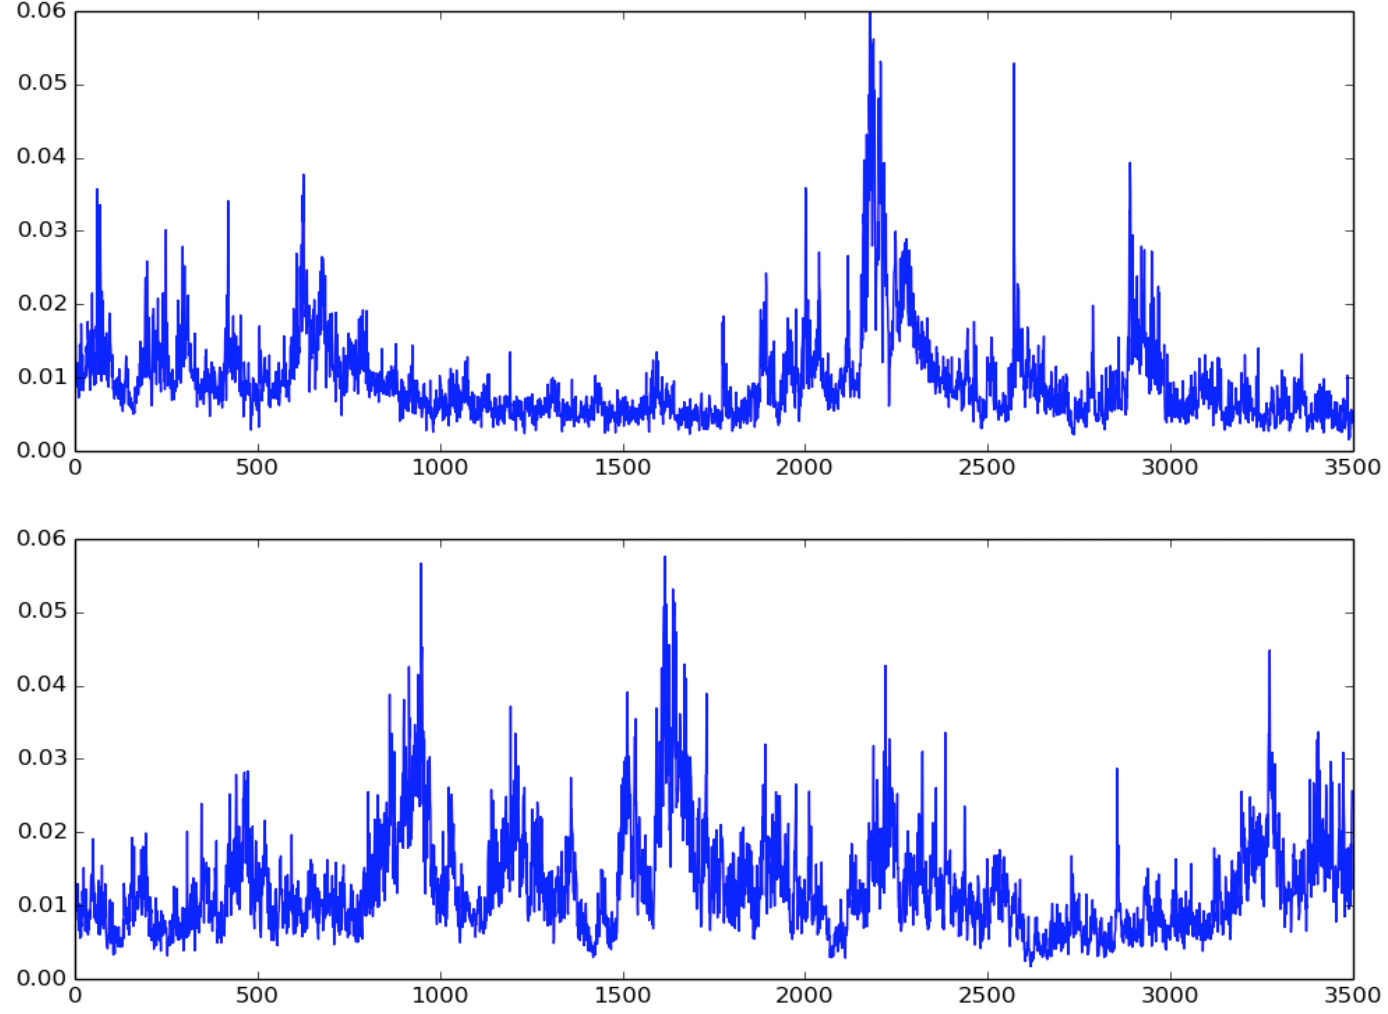
\includegraphics[width=0.85\textwidth ]{figs/gatheral_2014_fig36_p22}
    \caption{Extracted directly from Gatheral et al., 2014, \cite[Figure~3.6]{gatheral2014volatility}. Sample path of the model generated volatility (bottom) compared with the S\&P volatility (top). The x-axis represents the time to maturity in days, and the y-axis represents volatility.}
    \label{fig:gatheral_2014_volplots}
\end{figure}
\\

As is highlighted in \cite{gatheral2014volatility}, we see a striking similarity between both plots of Figure \ref{fig:gatheral_2014_volplots}, with both exhibiting periods of high volatility, followed or preceded by periods of low volatility. Recall that choosing $H<1/2$ means that the increments of the fractional Brownian motion are negatively correlated. In this analysis, $H$ was chosen to be less than 1/2 which would capture this certain trend in the model, as was discussed in Section \ref{sec:fractionalBm}. The smoothness of the volatility process could be captured through this model by tuning $H$.

It is important to mention that RFSV model is not long memory. However, when applying standard statistical estimators to data simulated by the RFSV model, long memory was incorrectly found to be present, with parameters estimated similar to those found in other studies. This led Gatheral et al. to conclude that this is why volatility having a long memory property is often accepted as a stylised fact. 

A more recent paper \cite{fukasawa2020volatility} also showed that volatility has to be rough through an arbitrage argument, involving the power law associated with implied volatility which is empirically observed in option markets \cite{Carr2001}. The power law of implied volatility, also known as the 'volatility smirk', aims to approximate the implied volatility curve of some options, which have a higher implied volatility for low strikes and a lower implied volatility for higher strikes. This shape is shown to be a negative skew, where the curve is steep for low strikes and flattens out for higher strikes (hence the name 'volatility smirk'). Fukusawa \cite{fukasawa2020volatility} shows that there is an arbitrage opportunity if volatility isn't rough given an option market obeying the power law given in Equation \ref{eqn:powerlaw},

\begin{equation}
\label{eqn:powerlaw}
\frac{\sigma_{BS}(K,T) - \sigma_{BS}(K',T)}{K-K'}\propto T^{H-1/2}
\end{equation}
where K \approx 0$, $K' \approx 0$, with $H \approx 0$ when $T \approx 0$. Here, $\sigm$a_{BS}(K,T)$ is the Black-Scholes implied volatility with log-moneyness $K$ and time to maturity T. This arbitrage opportunity is under the assumption that the asset price is a positive continuous It\^o semi-martingale.

Further studies have explored the origin of rough volatility, and it is considered to be a consequence of the no arbitrage principle and market impact \cite{jusselin2018noarbitrage}. In this context, market impact is defined to be the fact that on average for a given asset, a buy order increases it's price and a sell order causes a decrease in it's price. Given the overwhelming evidence discovered through such studies, it has been thoroughly accepted as a stylized fact that volatility is indeed rough.

\subsection{Pricing with rough volatility}

%Stochastic models such as Hull and White, Heston, and SABR are criticised for generating implied volatility surfaces whose shapes differ substantially from those observed empirically in the market. 

In this section, we describe how Rough Fractional Stochastic Volatility models can be used to price contingent claims and thus for option pricing. We first discuss the method of pricing under the physical measure $\mathbb{P}$, and then under the risk-neutral measure $\mathbb{Q}$. 

\subsubsection{Pricing under P}

As stated in the previous section, the distribution of increments of the logarithm of realized variance were found to be close to Gaussian, which motivates the use of a model where $\sigma_{t}$ is treated as a lognormal random variable. The time series of the realised variance was proposed to be modelled by:

\begin{equation}
\label{eq:realizedvariance}
    log\sigma_{t+\Delta} - log\sigma_{t} = \nu (W_{T+\Delta}^{H} - W_{t}^{H})
\end{equation}

where $W^{H}$ is fBM.
Now, consider the Mandelbort-Van Ness representation of fBM $W_{H}$:

$$W_{t}^{H} = C_{H} [\int_{-\infty}^{t} \frac{dW_{s}^{P}}{(t-s)^{\gamma}} - \int_{-\infty}^{0} \frac{dW_{s}^{P}}{(-s)^{\gamma}}]$$


If we substitute the previous equation into (\ref{eq:realizedvariance}), then the evolution of the instantaneous variance $\nu_{u}$ under the physical measure P would be:
\begin{equation}
\label{eq:realizedvariance}
    log\upsilon_{u} - log\upsilon_{t} := 2  \nu [M_{t}(u) + Z_{t}(u)]
\end{equation}

Let introduce $\tilde{W_{t}^{P}(u)}$ which has the same properties as $M_{t}(u)$:

\begin{equation}
    \tilde{W_{t}^{P}(u)}:= \sqrt{2H} \int_{t}^{u} \frac{dW_{s}^{P}}{(u-s)^\gamma}
\end{equation}

With $\eta := 2 \nu C_{H}/ \sqrt{2H}$ we have $2\eta C_{h} M_{t}(u) = \eta \tilde{W_{t}^{P}(u)}$, so we can write the instantaneous variance as:
\begin{equation}
\label{eq:volunderP}
\begin{split}
    \upsilon_{u} & = \upsilon_{t} exp (\eta \tilde{W_{t}^{P}(u)} + 2\eta C_{H} Z_{t}(u)) \\
    & = \mathbb{E}^{P} [\upsilon_{u}| \mathcal{F}_{t}] \varepsilon (\eta \tilde{W_{t}^{P}(u)})]
\end{split}
\end{equation}
 
 which is defined using two standard Brownian motions $Z_{P}$ and $W_{P}$ with a constant correlation $\rho$. We can also see that the conditional distribution of $\upsilon_{u}$ depends on $\mathcal{F}_{t}$ but only through the variance forecasts $^{P} [\upsilon_{u}| \mathcal{F}_{t}]$. Therefore, in order to price options, we do not need to know the $\mathcal{F}_{t}$.

It is important to recall that the dynamic of the price would be:

\begin{equation}
     \frac{dS_{u}}{S_{u}} = \mu_{t} du + \sqrt{\upsilon_{u}}dZ_{u}^{P},
\end{equation}

\subsubsection{Pricing under Q}
\\

To price options we need an equivalent martingale measure such that the discounted prices process $S_{t}$ is a martingale under this new measure, i.e changing from measure P to measure Q.
\\

The following changes of measure are done:

\begin{equation}
    dZ_{u}^{Q} = dZ_{u}^{P} + \frac{\mu_{u}}{\sqrt{\upsilon_{u}}}du
\end{equation}

where $ t \leq u \geq T$.

\begin{equation}
    dW_{u}^{Q} = dW_{u}^{P} + [\rho \mu_{u} / \sqrt{\nu_{u}} + \rho \gamma_{u}] du
\end{equation}

In fact, let consider a general change of measure of the style:

$$dW_{s}^{P} = dW_{s}^{Q} + \lambda_{s} ds$$

where $\gamma$ can be interpreted as the price of volatility risk. In this sense, we can rewrite (\ref{eq:volunderP}) as:

\begin{equation}
\label{eq:volunderQ}
    \upsilon_{u} & = E^{P} [\upsilon_{u}| \mathcal{F}_{t}] \varepsilon ( \eta \tilde{W_{t}^{Q}}(u)) exp [\eta \sqrt{2H} \int_{t}^{u} \frac{\lambda_{s}}{(u-s)^{\gamma}} ds]
\end{equation}

\\

\subsection{Bergomi Rough model}

In this subsection, the Bergomi model is transformed into a Rough Bergomi Model, which has showed to fit the SPX volatility better than conventional Markovian stochastic models \cite{Bayer2016pricing}.

A relevant characteristic which distinguish among volatility models is the term structure of the ATM volatility skew, defined as:

\begin{equation}
    \psi(\tau) = \lvert \frac{\partial}{\partial k} \sigma_{BS}(k,\tau) \rvert_{k = 0}
\end{equation}

where $\tau = T - t$ is the time to maturity, and $k$ is the log-moneyness equal to $log(\frac{K}{S_{t}})$. Stochastic models present the ATM volatility skew to be constant for short dates and inversely proportional to $\tau$ for long dates. In fact, evidence has showed that skew volatility is proportional to $\tau^{-\alpha}$, for $0\geq \alpha \leq 1/2$. 
\\

\begin{figure}[htpb]
    \centering
    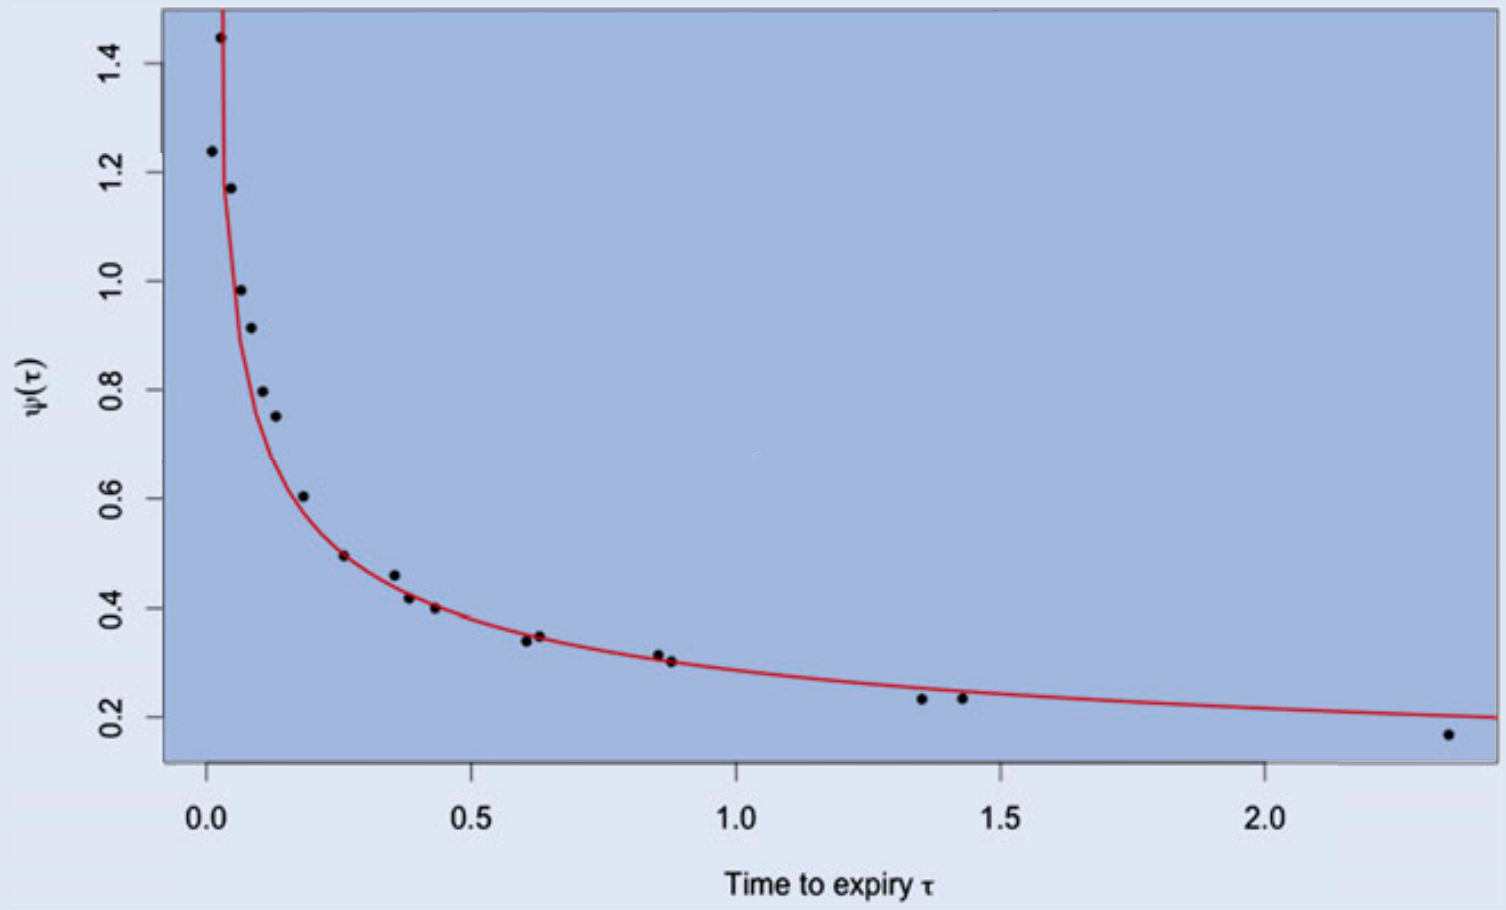
\includegraphics[width=0.85\textwidth ]{figs/Bayer2016_fig2.png}
    \caption{Extracted from Bayer et al., 2016  \cite[Figure~2]{Bayer2016pricing}. Plot shows change in volatility skew $\psi(\tau)$ with respect to $\tau$, time to expiry.measured in years The points are non-parametric estimates of the S\&P ATM volatility skews as of 14/08/13. Red curve is the power-law fit $\psi(\tau) = A\tau^{−0.407}$, where $\tau$.}
    \label{fig:gatheral_2014_volplots}
\end{figure}
\\

Bergomi and Guyon (2012) derive a small noise expansion for the smile in a stochastic volatility model making use of a forward variance curve, where forward variance is defined as the expectation under the pricing measure of the future instantaneous variance. In this way, given a stochastic model written in the forward curve form, the term structure of ATM skew can be computed easily. The n-factor Bergomi variance curve model can be written as:

\begin{equation}
\label{eq:Bergomimodel}
    \xi_{t}(u) = \xi_{0}(u) \epsilon(\sum_{i=1}^{n} \eta_{i} \int_{0}^{t} e^{-K_{i}(u-s) dW_{s}^{i}})
\end{equation}

where $\epsilon_{.}$ denotes the stochastic exponential and $\xi_{0}(.)$ denotes the initial forward variance curve. In this case, the Bergomi model generates a term structure volatility skew of the form:

$$\sum_{i=1}^{} \frac{\eta_{i}}{K_{i}} (1- \frac{1-e^{-K_{i}} \tau}{{K_{i}} \tau})$$

Thus, to generate the empirically observed form of $\tau^{-\alpha}$ it is expected to replace the exponential kernels in (\ref{eq:Bergomimodel}) with a power-law kernel. Thus, we end up with the rBergomi model which can be simulated as:

\begin{equation}
    S_{t} = S_{0} \epsilon (\int_{0}^{t} \sqrt{\nu_{u}} dZ_{u})
\end{equation}
\begin{equation}
    \nu_{u} = \xi_{0}(u) \epsilon( \eta_{i} \sqrt{2H} \int_{0}^{u} \frac{1}{(u-s)^{\gamma}} dW_{s})
\end{equation}

The rBergomi model is a non-Markivian generalization of the Bergomi model. This model consists of only three parameters: $H, \eta$ and $\rho$, where the later represents the correlation between volatility moves and prices moves. The parameters mentioned can be interpreted as:
%https://mfe.baruch.cuny.edu/wp-content/uploads/2018/02/RoughVolatilityColumbia2018.pdf

\begin{itemize}
    \item $H$ controls the decay of ATM skew for very short maturities.
    \item $\rho \eta$ defines the level of ATM skew for longer maturities.
    \item keeping $\rho \eta$ but decreasing $\rho$, towards to be negative, makes the minimum of each smile move to higher strikes.
\end{itemize}

In figure \ref{fig:Rough_vol_columbia_fig8}, it is shown how rBergomi model fits the SPX option market. The data was taken on Wednesday prior to expiration of the given options, in order to make the shortest expiration smile more meaningful. Parameters chosen for this day were: $H = 0.05, \eta = 2.3$ and $\rho = -0.9$. It is impressive how only using three parameters, we could get a good fit of the whole SPX volatility surface. It is worth to mention, that rBergomi model did pretty well for extreme short-dated smile and there was no necessity of adding jumps.

\begin{figure}[htpb]
    \centering
    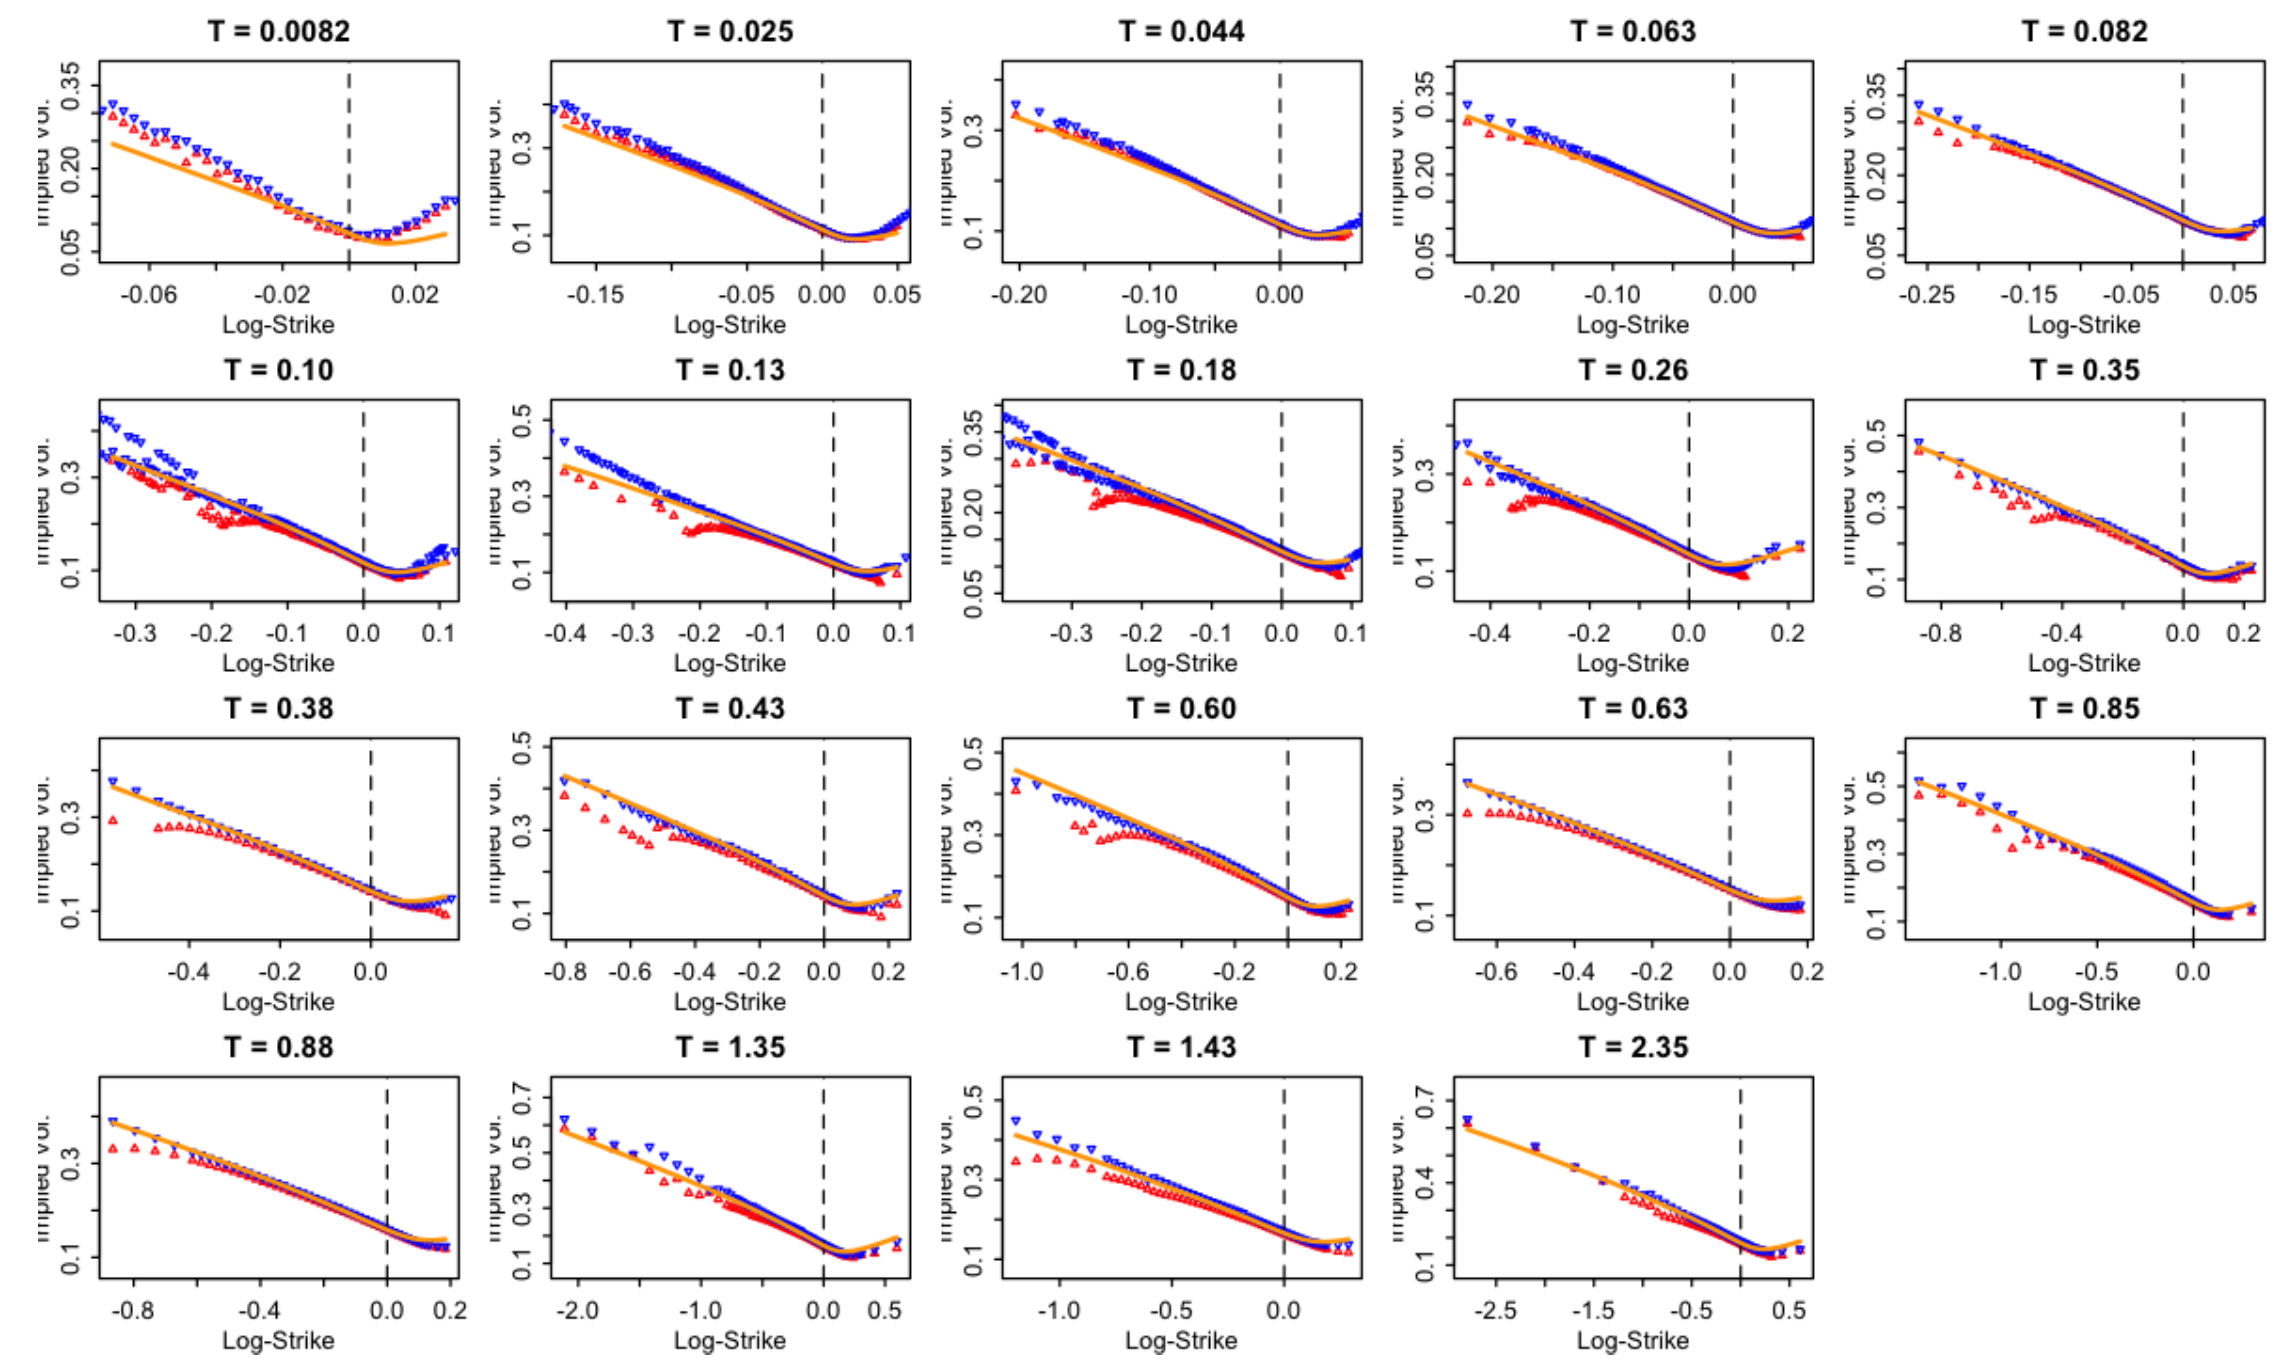
\includegraphics[width=1.0\textwidth ]{figs/Rough_vol_columbia_fig8}
    \caption{Extracted from Gatheral (2017) presentation to Baruch college \cite[Figure~8]{Rough_vol_columbia}. Comparison of implied volatilities of SPX and rBergomi model. Red points represent the bid offer, blue points represent the ask offer and orange lines correspond to the rBergomi simulation.}
    \label{fig:Rough_vol_columbia_fig8}
\end{figure}

\subsection{The Rough Heston volatility Model}
\label{sebsec:rough_heston}
The classical Heston model has been introduced, as have the pitfalls  of these simplistic early option pricing models. The classical Heston model does not agree with time series in practice, and does not generate a volatility surface similar to that observed. However, there are flexibility benefits to a model with additional parameters, particularly when applying a rough volatility framework. Small Hurst parameters & fBM are introduced, and the Ricatti characteristic function can be replaced with with a fractional Ricatti characteristic function to form the rough Heston model, producing behaviour seen in both historical & implied volatility. This has been well discussed in \cite{OElEuch2018} and \cite{ElEuchRosenbaum19}.
\\

Before describing why Rough Heston models produce accurate implied volatility models, we must first introduce Hawkes process. A Hawkes process is a class of stochastic process, pleasantly articulated in \cite{laub2015hawkes}, which has a "self-exciting" characteristic, whereby each time step, or "arrival" over time, within a process leads to excitement which gives a greater probability of exaggerating the characteristics of the process experienced at current time step in the subsequent time step. When a Hawkes process is interpreted as a model of a tradeable asset price over time, it is clear to see how this can be successfully applied to the fickle behaviors of financial market. I.e., where large volumes of sales/buying of an asset leads to further selling/buying, and the resulting sensational decrease/increase of the asset price. This behaviour is most famously seen in large financial crashes (the 2008 financial crisis, Brexit, flash crash of 2010), or short term economic bubbles, and can be seen in Figure \ref{fig:gatheral_2014_volplots}. 
\\

By sequencing a large number of Hawkes type point processes in \cite{omar2016microstructural}, it was found that these converge to a rough Heston model over the long run, with careful construction considerations. Micro-structures of the rough Heston were created via ultra-high-frequency Hawkes style price model sequences using the following stylised facts of the modern markets: 
\begin{enumerate} 
\item The majority of orders in the market are reactive algorithmic trades with no true economic rationale (described as highly endogenous). 
\item Arbitrage scenarios are highly unlikely due to the high frequency nature of the orders made in the market.  
\item Large algorithmic transactions, split over time and not in one order, make up a large proportion of transactions in the market.
\item There is bid-ask asymmetry: markets shall react differently to a market maker selling an asset as opposed to buying. The price in the market of a given asset shall likely increase when a market maker buys this asset, however the change in the assets market price is likely to be of greater (negatively) upon a market maker selling this asset. This is a result of the availability of this asset in the market reduces upon a buying, but increases when sold.  
\end{enumerate}
\\

Prior to defining the Rough Heston model we must return to the fBM in \ref{sec:fractionalBm} and $(\textit{$W^H_t$})$, with Hurst parameters $\textit{H} \in (0,1)$, from Section  \ref{sec:rough_vol_evidence}, to be represented in the Mandelbrot - Van Ness representation:
\\

\begin{equation}
\label{eqn:MvN_Hurst}
{W^H_t} = \frac{1}{\Gamma(H + \frac{1}{2})} \int_{0}^{-\infty} ((t-s)^{H-\frac{1}{2}} - (-s)^{H - \frac{1}{2}})W^H_s + \frac{1}{\Gamma(H + \frac{1}{2})} \int_{0}^{-\infty} (t-s)^{H-\frac{1}{2}}W^H_s
\end{equation}
We can see how influential  the kernel  $(t-s)^{H-\frac{1}{2}}$ is within rough volatility dynamics when $H<\frac{1}{2}$, and that the process,
$$\int_{0}^{-\infty} (t-s)^{H-\frac{1}{2}} dW^s$$
has Holder regularity for $H - \epsilon$, for any $\epsilon>0$. El Euch et al.incorporated this kernel, $(t-s)^{\alpha-1}$, to the classical Heston model to introduce a rough volatility-type model, defining the rough Heston Model.
\\

\begin{equation}
\label{eqn:rough_heston}
v_t = v_0 + \frac{1}{\Gamma(\alpha)} \int_{0}^{t} (t-s)^{\alpha-1} \kappa (\theta - v_s)ds + \frac{1}{\Gamma(\alpha)} \int_{0}^{t} \xi\sqrt{v_s}dW_s^{v}
\end{equation}
\\

Where $\alpha = H+\frac{1}{2}$ and $\kappa, \theta, v_0$ and $\xi$ are all positive, and $\rho$ continues to be the correlation coefficient of the two Brownian motions and are all equivalent to Equation \ref{eqn:classic_heston_var}. This model was found to be well defined when ${\alpha} \in (\frac{1}{2},1)$ the volatility trajectories almost surely have Holder regularity $\alpha - \frac{1}{2} -\epsilon$, as for Equation \ref{eqn:MvN_Hurst}, where for any $\epsilon>0$. It is important to note that when $\alpha$ = 1 we achieve the classical Heston Model.
\\

To continue with a selected Hurst parameter of $H < \frac{1}{2}$ as per Gatheral et al.  \cite{gatheral2014volatility}. The Rough Heston model will be non-Markovian and $v_t$ is no longer a semi-martingale, which as stated \ref{sec:fractionalBm} introduces smoothness to the model. This provides perfect motivation for El Euch et al., to design micro-structures of Hawkes point processes to model the "nearly unstable" behaviour of past events, and go on to demonstrate that combining the convergence results of these processes yield the characteristic function of the log-price of the rough Heston model. The suitability of these results can be seen in Figure \ref{fig:elEuch_1}.
\\

\begin{figure}[htpb]
    \centering
    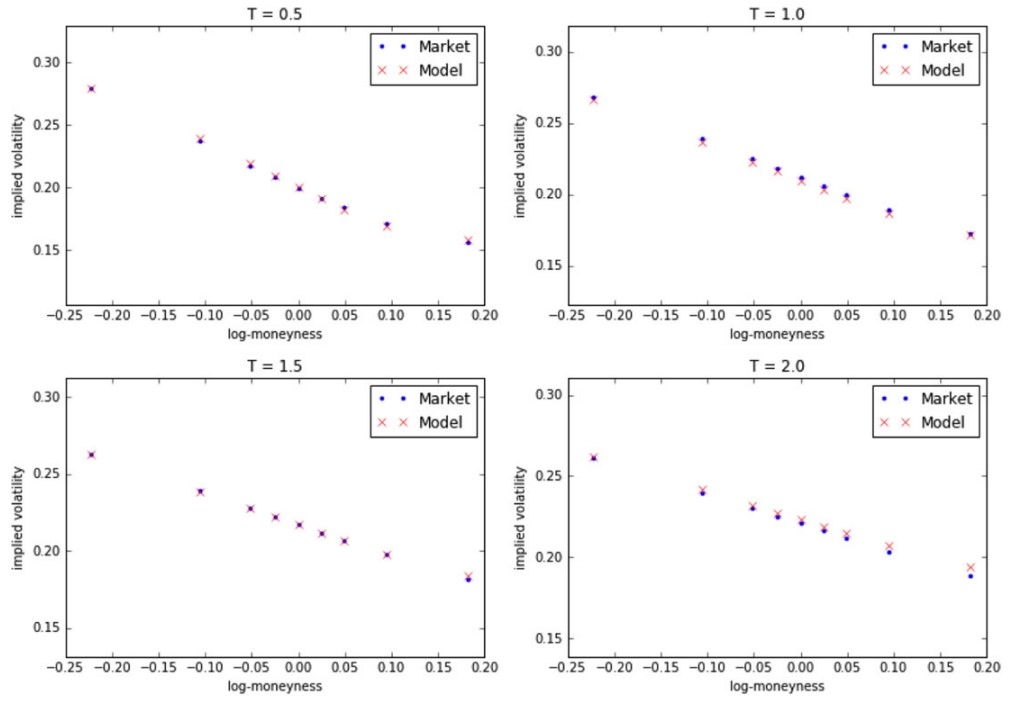
\includegraphics[width=0.85\textwidth ]{figs/elEuch_1.jpg}
    \caption{Extracted directly from El Euch and Rosenbaum, 2016, \cite[Figure~5.1]{omar2016microstructural}. Implied volatility surface generated from a rough Heston model with careful calibration ($\alpha=0.62$)has been shown to have miraculously close approximation to historical volatility on S\&P (January 2010) for varying maturity dates (T).}
    \label{fig:elEuch_1}
\end{figure}
\\

One additional note on the suitability of the rough Heston model is that the  "self-exciting" characteristics which the Hawkes micro-processes which jump in probability based on past events negates considerations of introducing any "jump processes", which are generally discouraged in modern models. 
\\

\section{Computational Advancements}
\label{sec:comp_advancement}

Moving to a generalised setting, we now focus on rough volatility models in general that we know are driven by fBM. As mentioned in \cite{jacquier2020deep}, the use of fBM in such models carries a computational burden with it. In terms of option pricing, this restricts the use of several pricing tools such as the Black-Scholes formula and other pricing PDE's, due to the non-deterministic nature of the volatility process.  Pricing via Monte Carlo simulation of the asset price and volatility processes is perhaps the one pricing tool that functions well, but it can be slow in approximating continuous time solutions within a sufficient level of accuracy. This is particularly true for simulating non-Markovian processes due to the extra memory required to store previous process states. Here, we give a brief overview of some work that introduces potential ways to combat the computational expense of exact Monte Carlo simulation of the volatility process. Namely, we discuss the Hybrid scheme in \cite{Bennedsen_2017}, the Markovian representation of fBM in \cite{harms2020strong} and the extension of the Donsker theorem to fBM in \cite{horvath2019functional}. These methods were introduced to improve the efficiency of the simulation of fBM and rough volatility processes while maintaining good levels of accuracy.

\subsection{The Hybrid Scheme}
\label{subsec:hybrid_scheme}
The Hybrid Scheme was introduced in \cite{Bennedsen_2017} in which they study simulation methods for Brownian semistationary processes. A Brownian semistationary process is given by Equation \ref{eqn:semistationary}. 

\begin{equation}
\label{eqn:semistationary}
X(t)=\int_{-\infty}^t g(t-s) \sigma(s) dW(s),  \ \  t\in\mathbb{R}
\end{equation}

Where $\sigma$ is a predictable process with respect to the given filtration. It is mentioned in \cite{Bennedsen_2017} that when $g(x) \propto x^\alpha$ and $\alpha \in (-\frac{1}{2}, \frac{1}{2}) \setminus \{0\}$, the process behaves (locally) like a fBM with Hurst parameter $H=\alpha+1/2$.  Therefore, being able to efficiently simulate such a process would help to improve computational efficiency for pricing in some rough volatility models.  

The Hybrid scheme involves approximating the function $g$ using a step function except for near 0, where a power function is used for approximation. Through a series of derivations, the resulting discretisation scheme is written as a linear combination of a Riemann sum and Wiener integrals. The scheme is given by Equations
\ref{eqn:hybrid1}-\ref{eqn:hybrid4}.  
\begin{equation}
\label{eqn:hybrid1}
X_n(t) = \hat{X}_n(t) + \tilde{X}_n(t)
\end{equation}
where,
\begin{equation}
\label{eqn:hybrid2}
\hat{X}_n(t) = \sum_{k=1}^{\kappa} L_g(\frac{k}{n}) \sigma (t-\frac{k}{n}) \int_{t-\frac{k}{n}}^{t-\frac{k}{n}+\frac{1}{n}}(t-s)^\alpha dW(s),
\end{equation}
and,
\begin{equation}
\label{eqn:hybrid3}
\tilde{X}_n(t)=\sum_{k=\kappa+1}^{N_n}g(\frac{b_k}{n})\sigma(t-\frac{k}{n})(W(t-\frac{k}{n}+\frac{1}{n})-W(t-\frac{k}{n})),
\end{equation}
with $L_g$ chosen so that,
\begin{equation}
\label{eqn:hybrid4}
g(t-s) \approx (t-s)^\alpha L_g(\frac{k}{n}), \ \ t-s \in [\frac{k-1}{n},\frac{k}{n}]
\end{equation}

The key takeaway from Equations \ref{eqn:hybrid1}-\ref{eqn:hybrid4} is to highlight that the scheme is driven by a Wiener process and not fBM, meaning that we retain the Markovian property. In terms of applying the scheme to rough volatility models, the Hybrid Scheme was used for option pricing in the Bergomi model via Monte Carlo simulation, as is discussed in the referenced paper. Using the Hybrid Scheme in this setting simplified the simulation process and reduced the computational cost compared to producing exact simulations from the model \cite[Page~20]{Bennedsen_2017}. The results from using the scheme were then compared to exact results from the Bergomi model and it showed that the Hybrid Scheme was able to produce almost exactly the same volatility smile as that produced by exact simulation from the Bergomi model while being significantly more efficient.

\subsection{Markovian Representation of fBM}
\label{subsec:markovian_rep_fBm}
Without going into too much detail, it was shown in \cite{harms2020strong} that fBM can be approximated by a Markovian representation consisting of the sum of $n$ weighted Orstein-Uhlenbeck processes.  Based on a set of assumptions outlined in the paper, the approximation is given by Equation \ref{eqn:markov_approx}.

\begin{equation}
\label{eqn:markov_approx}
W_t^{H,n} = \sum_{i=1}^n w_{n,i} \int_0^t e^{-(t-s)x_{n}n,i}dW_s, \ \ t \in [0,T] 
\end{equation}

where the $x_{n,i}$ are so-called 'speeds of mean reversion' and the $w_{n,i}$ are weights, with both terms taking positive values. This approximation forms part of a theorem which states that fBM is approximated by this representation at a rate of $n^{-r}$ for any given $r>0$. This theorem also states that under this approximation, put prices in the Bergomi model also converge at a rate of $n^{-r}$. 

Again, the key takeaway here is that a discrete Monte Carlo scheme for the rough Bergomi model can be achieved and since the representation is Markovian, it improves efficiency. It is also mentioned that in terms of error and complexity, this method outperforms several other computational methods. However, it is outperformed by the Hybrid Scheme that was discussed earlier. 

\subsection{Extension of Donsker's Theorem to fBM}
Like the previous examples, the motivation of extending Donsker's theorem for Brownian motion to fBM is to be able to approximate fBM in a way that would reduce computational cost. To give some context,  we state Donsker's Theorem.

 \noindent\textbf{Theorem (Donsker)}: \emph{Let} $\epsilon_1,...,\epsilon_n$ \emph{be i.i.d. random variables with mean 0 and variance} $\sigma^2$. \emph{Then for} $X^{(n)}$ defined by
 \begin{equation}
 \label{eq:donsker_thm}
 X_t^{(n)} = \frac{1}{\sigma \sqrt{n}} (S_{\lfloor nt \rfloor} - (nt - \lfloor nt \rfloor) \epsilon_{\lfloor nt \rfloor + 1}), \ \ t\in[0,1]
 \end{equation}
 where,
\begin{equation}
S_m = \sum_{i=1}^i \epsilon_m
\end{equation}

then $X_t^{(n)} \rightarrow W_t$ \emph{in distribution for} $t\ge0$ \emph{on the space of continuous functions, where} $W_t$ \emph{is classical Brownian motion}.

By being able to extend this theorem to fBM, one could approximate it using i.i.d. sequences of random variables leading to a simplified simulation process. Again, without going into too much detail, an extension of this theorem was provided in \cite{horvath2019functional}, approximating the logarithm of the stock price under a rough volatility model, under the assumption that the i.i.d. random variables have a finite second moment (variance in this case) and a number of other conditions. In terms of pricing, this approximation could then be applied to fractional binomial trees, which opens the door to pricing American-type options under rough volatility models. However, the branches of such trees generally do not recombine which adds to the complexity of this pricing method.   

\subsection{Further Advancements}
\label{subsec:tech_advancement}
In addition to the aforementioned numerical approximations, we also give a brief over view of the accompanying technological improvements that have also had a significant contribution to the improvements in pricing under rough volatility models. 

 Due to ongoing improvements in technological availability and computational power, making methods such as that presented by
 Horvath et al., \cite{horvath2019deep} increasingly accessible. 
 In this work it is shown that neural networks have a significant impact on the computational burden presented by the simulation of rough volatility processes. The authors show that a speed up factor of approximately 12,500 (on average) can be achieved when using neural networks as opposed to vanilla (ICE) Monte Carlo methods when calibrating parameters for rough volatility models. They also show that the neural network approach generalises very well to all types of rough volatility models. 
 Due to the model speedup achieved by the use of neural networks, model calibrations can be achieved on the order of seconds, or milliseconds as is shown in Figure \ref{fig:Horvath_fig10_11}. This means that calculations of rough volatilities and model calibration can be done in a real-time, and pricing is fast enough to use either gradient, or gradient free methods.
 
 \begin{figure}[htpb]
    \centering
    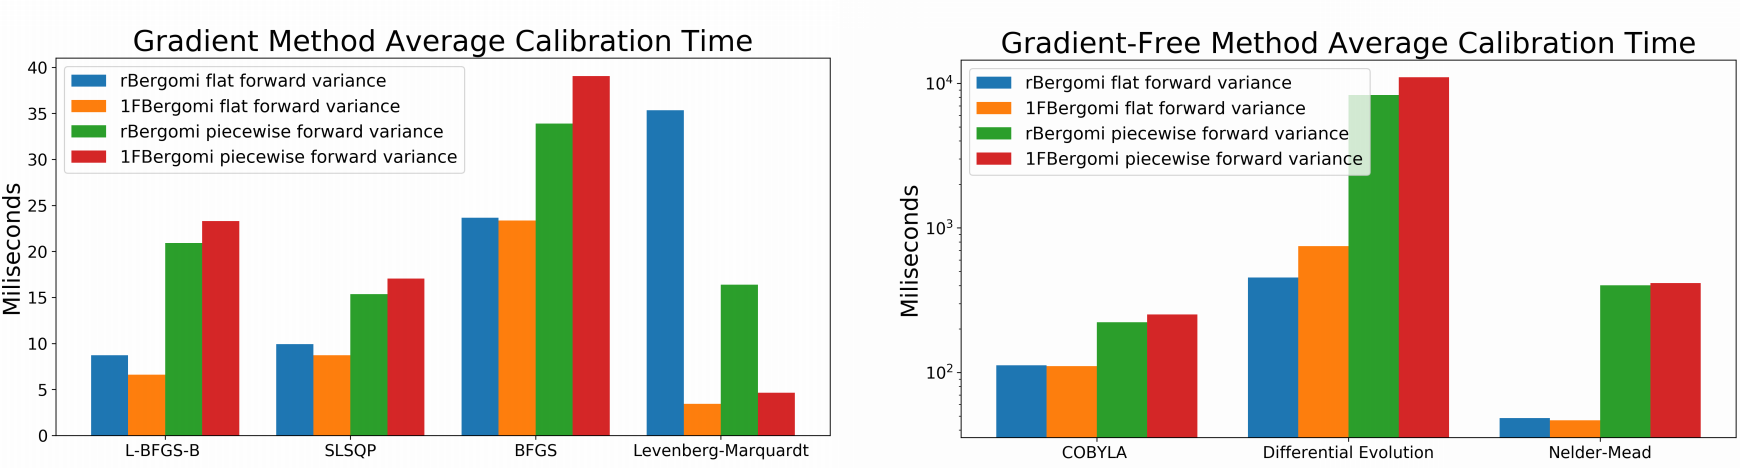
\includegraphics[width=1.0\textwidth ]{figs/Horvath_fig10_11}
    \caption{Extracted directly from Horvath et al., 2014, \cite[Figures~10\&11]{horvath2019deep}. Plots show that model calibration takes on the order of seconds/milliseconds for both gradient and Gradient-free methods.}
    \label{fig:Horvath_fig10_11} 
\end{figure}

\section{Summary and Future work}
\label{sec:conclusion}
 
We have described here how models that contain rough volatility are much more accurate pricing tools, than those where volatility is constant or deterministic. The models we considered here are by no means exhaustive, but we focused primarily on the more popular models for brevity and clarity. 

We describe here how log volatility behaviour is well described as a fractional Brownian motion, with a Hurst parameter less than 1/2. The models we have looked into here were generally known to be good representations of volatility, however due to the considerable computational resources required were not well adopted by industry. We have illustrated here how improvements in numerical methods such as use of a hybrid scheme, a Markovian representation of fBm, and extensions to Donsker's theorem have significantly helped in making this rough volatility far more accessible. 


% In the vast majority of papers this section is not present. It could be used to provide a brief summary of the paper or some areas for further research. Most likely it won't be useful for the final essays.

% The final point in this document is of high importance. 

\bibliographystyle{amsrefs}
%  \bibliographystyle{plain}  % Or use the `amsrefs' package (http://www.ams.org/tex/amsrefs.html)!
\bibliography{my_bibtex_file.bib}
 \addcontentsline{toc}{section}{Bibliography}
\end{document}
